\documentclass[12pt,a4paper]{report}
\usepackage[T1]{fontenc}
%adjust your page margins here
\usepackage[top=0.70in, bottom=0.70in, left=0.8in,right=0.80in]{geometry} % setting the page alignment with this package
\usepackage[pdftex]{graphicx} %for embedding images
\usepackage[%dvips, % commented for pdflatex
bookmarks,  colorlinks=false]{hyperref} %for creating links in the pdf version and other additional pdf attributes, no effect on the printed document
\hypersetup{%
    pdfborder = {0 0 0}
}
\usepackage[final]{pdfpages} %for embedding another pdf, remove if not required
\usepackage{float} %used for figure placement with H as a parameter
\usepackage{hyperref}
\usepackage{pslatex} % for times new roman, old package, but works
\usepackage{array} % for making text bold in table
\usepackage{setspace}
\usepackage{float}
\usepackage{enumerate}
\usepackage{longtable}

\usepackage[font=small,labelfont=bf]{caption}
\def\figurename{\textbf{Figure }}

\usepackage{listings}
\usepackage{color}

\definecolor{dkgreen}{rgb}{0,0.6,0}
\definecolor{gray}{rgb}{0.5,0.5,0.5}
\definecolor{mauve}{rgb}{0.58,0,0.82}
 
\lstset{ %
  language=Java,                % the language of the code
  basicstyle=\footnotesize,           % the size of the fonts that are used for the code
  numbers=left,                   % where to put the line-numbers
  numberstyle=\tiny\color{gray},  % the style that is used for the line-numbers
  stepnumber=1,                   % each line is numbered
  numbersep=5pt,                  % how far the line-numbers are from the code
  backgroundcolor=\color{white},      % choose the background color. You must add \usepackage{color}
  showspaces=false,               % show spaces adding particular underscores
  showstringspaces=false,         % underline spaces within strings
  showtabs=false,                 % show tabs within strings adding particular underscores
  frame=single,                   % adds a frame around the code
  rulecolor=\color{black},        % if not set, the frame-color may be changed on line-breaks within not-black text (e.g. commens (green here))
  tabsize=2,                      % sets default tabsize to 2 spaces
  captionpos=b,                   % sets the caption-position to bottom
  breaklines=true,                % sets automatic line breaking
  breakatwhitespace=false,        % sets if automatic breaks should only happen at whitespace
  title=\lstname,                   % show the filename of files included with \lstinputlisting;
                                  % also try caption instead of title
  keywordstyle=\color{blue},          % keyword style
  commentstyle=\color{dkgreen},       % comment style
  stringstyle=\color{mauve},         % string literal style
  escapeinside={\%*}{*)},            % if you want to add a comment within your code
  morekeywords={*,...}               % if you want to add more keywords to the set
}

%For the header and footer
\usepackage{fancyhdr}
\fancypagestyle{plain}{%
\fancyfoot[L]{\emph{Department of Computer Science and Engineering,SSNCE,Kalavakkam}} % except the center
\fancyfoot[R]{\thepage}
\renewcommand{\headrulewidth}{0.4pt}
\renewcommand{\footrulewidth}{0.4pt}
}

\pagestyle{fancy}

\rhead{\emph{WORKING WITH DJANGO FORMS}}

\fancyfoot[LO,LE]{\emph{Department of Computer Science and Engineering,SSNCE,Kalavakkam}}
\cfoot{}
\fancyfoot[RO, RE]{\thepage}
\renewcommand{\headrulewidth}{0.4pt}
\renewcommand{\footrulewidth}{0.4pt}
%For the header and footer Over

%Page Border
\usepackage{pgf}
\usepackage{pgfpages}

\pgfpagesdeclarelayout{boxed}
{
  \edef\pgfpageoptionborder{0pt}
}
{
  \pgfpagesphysicalpageoptions
  {%
    logical pages=1,%
  }
  \pgfpageslogicalpageoptions{1}
  {
    border code=\pgfsetlinewidth{2pt}\pgfstroke,%
    border shrink=\pgfpageoptionborder,%
    resized width=.95\pgfphysicalwidth,%
    resized height=.95\pgfphysicalheight,%
    center=\pgfpoint{.5\pgfphysicalwidth}{.5\pgfphysicalheight}%
  }%
}
\pgfpagesuselayout{boxed}
\setlength{\parindent}{1cm}

\usepackage{lastpage}
\usepackage{fancyhdr}
%\usepackage{ragged2e}
%\raggedright{\chead{\thepage\ of \pageref{LastPage}}}
%%% Remove the next line if you want the figures at their place    
\usepackage[figuresonly,nolists,nomarkers]{endfloat}
\usepackage{lipsum}
% Uncomment the following line for the final version
%\nofiles\renewcommand{\processdelayedfloats}{}

% Page numbering: top right
\usepackage{fancyhdr}

\pagestyle{fancy}
\fancypagestyle{plain}{

	\fancyhead[RO,RE]{\thepage\ of \pageref{LastPage}} %RO=right odd, RE=right even
	\renewcommand{\headrulewidth}{0pt}
	\renewcommand{\footrulewidth}{0pt}
}
\pagestyle{empty}
\pagenumbering{gobble}

%GLOBAL SETTINGS OVER, DOCUMENT BEGINS
\begin{document}
\renewcommand\bibname{References}
\lhead{ }

%FROM HERE YOUR PAGES START GETTING ADDED

% includes the cover page
\newpage
\begin{center}
\thispagestyle{empty}

\Large{\textbf{A PROJECT REPORT\\ \large{ON}}}\\[0.7cm]
\LARGE{\textsc {\textbf{WORKING WITH DJANGO FORMS}}}\\[0.5cm]
\vspace{0.5cm}
\Large{\textbf{\\Submitted to}}
\LARGE{\textbf{\\SSN College of Engineering\\}}
\vspace{1cm}
\Large{\textbf{\\BY}}\\[0.5cm]
\begin{table}[h]
\centering
\Large{
\begin{tabular}{>{\bfseries}lc>{\bfseries}r}
SUBALAKSHMI SHANTHOSI S & & 186001008 \\
\end{tabular}}
\end{table}
\vspace{0.5cm}
\large{\textbf{UNDER THE GUIDANCE OF}}\\
\large{\textbf{DR. R.S MILTON}}\\
\vspace{1cm}
\large{\textbf{DEPARTMENT OF COMPUTER SCIENCE AND ENGINEERING}}\\
\Large{\textbf{SSN COLLEGE OF ENGINEERING}}\\
\vspace{0.5cm}
\large{\textbf{Rajiv Gandhi Salai (OMR),Kalavakkam -- 603 110 }}
\large{\textbf{\\MAY-2019}}\\
\vspace{1cm}
\Large{\textbf{Sri Sivasubramaniya Nadar College of Engineering(SSNCE)\\}}
(An Autonomous Institution, Affiliated to Anna University, Chennai)\\
\newpage
\end{center}
\newpage

\newpage
\begin{center}
\vspace{5cm}
\thispagestyle{empty}
{\fontfamily{ptm}\selectfont
\Large{\textsc {\textbf{WORKING WITH DJANGO FORMS}}}}\\
\Large{\textbf{\\A PROJECT REPORT\\ ON}} \\[0.3cm]
{\fontfamily{ptm}\selectfont
\Large{\textsc {\textbf{WORKING WITH DJANGO FORMS}}}}\\

\Large{\textit{\textbf{\\Submitted by}}}

\vspace{1cm}
\begin{table}[h]
	\centering
	\Large{
		\begin{tabular}{>{\bfseries}lc>{\bfseries}r}
			SUBALAKSHMI SHANTHOSI S & & 186001008 \\
	\end{tabular}}
\end{table}
\vspace{0.5cm}
{\fontfamily{ptm}\selectfont
\large{\textbf{DEPARTMENT OF COMPUTER SCIENCE AND ENGINEERING}}}\\
\vspace*{0.5cm}
\Large{\textbf{SSN COLLEGE OF ENGINEERING}}\\
\large{\textbf{\\MAY-2019}}\\
\vspace{10cm}


\includegraphics[scale=0.35]{ssnLogoNew.png}

\Large{\textbf{Sri Sivasubramaniya Nadar College of Engineering\\}}
{(An Autonomous Institution, Affiliated to Anna University, Chennai)}\\
\end{center}
\newpage

% includes the certificate page
\begin{center}
\thispagestyle{empty}
\vspace{10cm}
\LARGE{\textbf{Sri Sivasubramaniya Nadar College of Engineering }} \\ 
\normalsize{(An Autonomous Institution, Affiliated to Anna University, Chennai)} \\
Rajiv Gandhi Salai (OMR), Kalavakkam - 603 110 \\
\vspace{2cm}

{\Huge \textbf{BONAFIDE CERTIFICATE }}\\[0.5cm]
\end{center}
\linespread{1.13}
\large{\centering{Certified \space  that \space this \space project\space report \space  titled,}
\textbf{...{``WORKING WITH DJANGO FORMS``}} \space is \space the \space bonafide \space work \space of \space \textbf{''SUBALAKSHMI SHANTHOSI S(186001008)....''} \space who carried out the project work under my
guidance. }\\[0.2cm]
\begin{spacing}{0}
\vspace{3.0cm}
\large{\textbf{SIGNATURE:}}\hspace*{2.5in}\large{\textbf{SIGNATURE:}}\\
\vspace*{1,5cm}

\hspace*{0.02in}\textbf{HEAD OF THE DEPARTMENT}\hspace*{0.85in}\textbf{SUPERVISOR}\\[2cm]
\vspace*{1,4cm}
Submitted for end semester project examination held on ........................\\[8cm]

\textbf{INTERNAL EXAMINER }
\end{spacing}
 
\newpage

% includes the acknowledgements page
\begin{center}
\thispagestyle{empty}
\LARGE{\textbf{Acknowledgements}}\\[1cm]
\end{center}
\linespread{1.13}
\large{\paragraph{}We are profoundly grateful to \textbf{Prof. GUIDE NAME} for his expert guidance
and continuous encouragement throughout to see that this project rights its
target since its commencement to its completion.}
\large{\paragraph{}We would like to express deepest appreciation towards \textbf{Dr. PRINCIPAL NAME},
Principal, NAME OF COLLEGE, \textbf{Prof. HOD NAME}, 
Head of Department of Computer Engineering and \textbf{Prof. PROJECT COORDINATOR NAME}, Project Coordinator whose
invaluable guidance supported us in completing this project.}
\large{\paragraph{}At last we must express our sincere heartfelt gratitude to all the staff members
of Computer Engineering Department who helped me directly or indirectly during this course of work.}
\begin{flushright}
{
GROUP MEMBER A\\
GROUP MEMBER B\\
GROUP MEMBER C\\
GROUP MEMBER D
}
\end{flushright}
\newpage
 
\newpage

\begin{center}
\thispagestyle{empty}
\vspace{2cm}

\LARGE{\textbf{ABSTRACT}}\\[1.0cm]

\end{center}
\thispagestyle{empty}
\large{\paragraph{} Working with django for designing customisable forms.\\
We begin by designing a basic form with primitive fields with in-build validation suite.Followed by creation of form it is been circulated to all the intended audience for filling whose responses are collected and stored in backstore.}
\large{\paragraph{}The user responses are presented to the creator of the form for viewing and filtering with specific requirements.}\\
\large{\paragraph{} Django functionality of building the \textbf{Model, Template and View (MTV) }} for ensuring separation of concern and enhanced useability in the development process. \\
Django's form functionality can simplify and automate vast portions of this work, and can also do it more securely than most programmers would be able to do in code they wrote themselves.\\

Django handles three distinct parts of the work involved in forms:\\
\begin{itemize}
	\item Preparing and restructuring data to make it ready for rendering.
	\item Creating HTML forms for the data.
	\item Receiving and Processing submitted forms and data from the client.
\end{itemize}
Django model describes the logical structure of an object, its behavior, and the way its parts are represented to us, a \textbf{Form} class describes a form and determines how it works and appears.\\

\vspace*{3cm}
\textbf{Keywords: }Form Design, Django-Form,Django Form Builder % adds the Research Methodology page
\newpage

%TABLE OF CONTENTS AND LIST OF FIGURES ARE AUTOMATICALLY ADDED BY FOLLOWING COMMANDS
%ADD FIGURE OF TABLES IF YOU NEED TO, CHECK DOCUMENTATION
\pagenumbering{roman} %numbering before main content starts


%To reset the Header & Footer for TOC and LOF
\pagestyle{empty}
\addtocontents{toc}{\protect\thispagestyle{empty}}
\tableofcontents % adds Index Page

\addtocontents{lof}{\protect\thispagestyle{empty}}
\listoffigures % adds List of Figures
\cleardoublepage

%And reset back the settings we choose for Header and Footer
\pagestyle{fancy}

\newpage
\pagenumbering{arabic} %reset numbering to normal for the main content

\chapter{Introduction}
\section{Working with Django Forms}
\subsection{Problem Statement}
\paragraph{} Modelling a form creation interface with basic form fields like - Integer,Character and Pick-List Fields for manipulation.\\

Separation of tight relationship with the model and that of a trivial form POST method by introducting customisation like : 
 
           \begin{enumerate}
           	\item Building Form with json fields.
           	\item Python code for data population in Models instead of manual entry.
           \end{enumerate}

\subsection{Requirements - Django Forms:}
The specific user and system requirements for building form creation interface are listed below :\\
\begin{enumerate}
    \item Creating Django forms which returns \textbf{structured data} on submission.
    \item End-to-end working of form submission flow.
    \item Customisation of form fields for enhanced useability.
    \item Including in-place form validation effortlessly.
    \item Customisation of form interface to handle JSON data.
    \item Population script to automate entries to the data store.
    
\end{enumerate}

 % adds the introduction page

\lstset{ %
	language=html,                % the language of the code
	basicstyle=\footnotesize,           % the size of the fonts that are used for the code
	numbers=left,                   % where to put the line-numbers
	numberstyle=\tiny\color{gray},  % the style that is used for the line-numbers
	stepnumber=1,                   % each line is numbered
	numbersep=5pt,                  % how far the line-numbers are from the code
	backgroundcolor=\color{white},      % choose the background color. You must add \usepackage{color}
	showspaces=false,               % show spaces adding particular underscores
	showstringspaces=false,         % underline spaces within strings
	showtabs=false,                 % show tabs within strings adding particular underscores
	frame=single,                   % adds a frame around the code
	rulecolor=\color{black},        % if not set, the frame-color may be changed on line-breaks within not-black text (e.g. commens (green here))
	tabsize=2,                      % sets default tabsize to 2 spaces
	captionpos=b,                   % sets the caption-position to bottom
	breaklines=true,                % sets automatic line breaking
	breakatwhitespace=false,        % sets if automatic breaks should only happen at whitespace
	title=\lstname,                   % show the filename of files included with \lstinputlisting;
	% also try caption instead of title
	keywordstyle=\color{blue},          % keyword style
	commentstyle=\color{dkgreen},       % comment style
	stringstyle=\color{mauve},         % string literal style
	escapeinside={\%*}{*)},            % if you want to add a comment within your code
	morekeywords={*,...}               % if you want to add more keywords to the set
}
\lstdefinestyle{base}{
	language=html,
	breaklines=true,
	basicstyle=\ttfamily\color{blue},
	moredelim=**[is][\color{red}]{@}{@},
}

\chapter{Introduction to HTML and CSS}
\section{HTML : Hyper Text Markup Language}
\subsection{Introduction to HTML}
\paragraph{} HTML is a \textbf{markup language} which tells how the computer should render a web page.\\ The documents themselves are plain text files with special "tags" or codes that a web browser uses to interpret and display
information on your computer screen. \\
\begin{itemize}
	\item Introduction
\begin{enumerate}
	\item An HTML file is a text file containing small markup tags.
	\item The markup tags tell the Web browser how to display the page.
	\item An HTML file must have an \textbf{htm} or \textbf{html} file extension. 
\end{enumerate}
    \item HTML Tags 
    \begin{enumerate}
    	\item HTML Tags are used to markup HTML elements.
    	\item HTML Tags are surrounded by < and > braces.
    	\item HTML Tags are either:
    	\begin{itemize}
    		\item Paired tags : Tags with opening and closing tags.
    		\item Closed tags : Tags without closing tag.
    	\end{itemize}
    \end{enumerate}
\newpage

\begin{table}[]
	\begin{tabular}{|l|l|l|ll}
		\cline{1-3}
		\textbf{Tag}   & \textbf{Description}           & \textbf{Example}                                                                                                                                                               &  &  \\ \cline{1-3}
		h1, . . . , h6 & Header tag                     & h1 to h6                                                                                                                                                                       &  &  \\ \cline{1-3}
		p              & paragraph element              & \textless{}p\textgreater{}Hi ...\textless{}/p\textgreater{}                                                                                                                    &  &  \\ \cline{1-3}
		span           & No line change after span      & \textless{}span\textgreater{}Hi...\textless{}/span\textgreater Bye.                                                                                                            &  &  \\ \cline{1-3}
		div            & Make division between contents & \textless{}div\textgreater content \textless{}/div\textgreater{}                                                                                                               &  &  \\ \cline{1-3}
		a              & Hyperlink in documents         & \textless{}a href ="\textless{}url\textgreater{}"\textgreater{}description\textless{}/a\textgreater{}                                                                          &  &  \\ \cline{1-3}
		center         & Move content to center         & \textless{}center\textgreater{}Centered  content \textless{}/center\textgreater{}                                                                                              &  &  \\ \cline{1-3}
		br             & Line break                     & \textless{}br\textgreater or \textless{}br/\textgreater{}                                                                                                                      &  &  \\ \cline{1-3}
		hr             & Horizontal line                & \textless{}hr\textgreater or \textless{}hr/\textgreater{}                                                                                                                      &  &  \\ \cline{1-3}
		pre            & Preserve formatting            & \textless{}pre\textgreater{}Preserved content\textless{}/pre\textgreater{}                                                                                                     &  &  \\ \cline{1-3}
		table          & Include a table                & \textless{}table\textgreater \textless{}tr\textgreater \textless{}td\textgreater{}TR One\textless{}/td\textgreater{}\textless{}/tr\textgreater \textless{}/table\textgreater{} &  &  \\ \cline{1-3}
	\end{tabular}
      \caption{HTML basic tags } \label{tab:sometab}
    
\end{table}
\item \textbf{HTML 5} \\
HTML 5 is backward compactible \\
\textbf{Features in HTML 5}:
\begin{enumerate}
	\item \textbf{New semantic elements} to allow us to define more parts of our markup unambiguously and
	semantically rather than using lots of classes and IDs. 
	
	\item \textbf{New elements and APIs} for adding video, audio, scriptable graphics, and other rich application
		type content to our sites.
	\item New features for standardising functionality that we already built in bespoke, hacky ways.\textbf{ Server sent updates and form validation } spring to mind immediately. 
	\item Customised handling of \textbf{markup errors}.
	\item Support for \textbf{Offline web pages}.
\end{enumerate}
\item \textbf{HTML 5 Design principles}:
\begin{enumerate}
	\item Ensuring support for existing content: Process existing HTML documents as HTML5 documents. 
	\item Degrading new features gracefully in older browsers:
	HTML5 should degrade gracefully in old or less capable agents.
	\item Not reinventing the wheel : "If it ain't broke, don't fix it."
	\item Paving the cow paths: Work with already build path. Embrace and adopt the de facto standards in the official specs.
	\item Evolution, not revolution: Evolve existing system than to replace it with another new standards.
\end{enumerate} 
\end{itemize}
\newpage
\subsection{Introduction to CSS}
\paragraph{}CSS is used to enhance the look of the web page.\\
Types of CSS styling:
\begin{itemize}
	\item Inline CSS : 
	\\ Style are defined inline to the individual tags:
\begin{lstlisting}[language=html]
<!-- css.html -->

<!DOCTYPE html>
<html>
<head>
<title>CSS Tutorial</title>
</head>

<body>

<h3 style="color:blue"> Heading 1 </h3>
<h3 style="color:red"> Heading 3 </h3>

</body>

</html>
\end{lstlisting}
\item Embedded CSS:
 Styles are specified within the <style> tag in HTML document.\\
 \begin{lstlisting}[language=html]
 <!-- cssEmbedded.html -->
 <!DOCTYPE html>
 <html>
 <head>
 <title>CSS Tutorial</title>
 <style type="text/css">
 h3.h3_blue{ /*change color to blue*/
 color: blue;
 }
 
 h3.h3_red{ /*change color to red*/
 color:red;
 }
 </style>
 </head>
 <body>
 <h3 class='h3_blue'> Heading 1 </h3>
 <h3 class='h3_blue'> Heading 3 </h3>
 <h3 class='h3_red'> Heading 1 </h3>
 </body>
 </html>
 \end{lstlisting}
 \item External CSS: Style document in css extension is written separately which are imported into the HTML document.
 
 \begin{lstlisting}[language=html,numbers=none,style=base]
 /* asset/css/my_css.css */
 h3.h3_blue{
 color: blue;
 }
 
 h3.h3_red{
 color:red;
 }
 \end{lstlisting}
 
 \begin{lstlisting}[language=html,numbers=none,style=base]
 <!-- CSS External -->
 <head>
 <title>CSS External file inclusion</title>
 <link rel="stylesheet" type="text/css" href="asset/css/my_css.css">
 </head>
 \end{lstlisting}

\end{itemize}
\begin{itemize}
	\item Basic CSS Selectors \\
	Three types of  selectors in CSS :  
	\begin{enumerate}
		\item \textbf{Element:}Can be selected using it's name e.g. 'p', 'div' and 'h1' etc.
		\item \textbf{Class:} Can be selected using '.className' operator e.g. '.h3\_blue'.
		\item \textbf{ID:}Can be selected using \#idName e.g. '\#my\_para'.
	\end{enumerate}
\begin{lstlisting}[language=html,style=base,numbers=none]
/* asset/css/my_css.css */
/*element selection*/
h3 {
color: blue;
}
/*class selection*/
.c_head{
font-family: cursive;
color: orange;
}

/*id selection*/
#i_head{
font-variant: small-caps;
color: red;
}
\end{lstlisting}
\begin{lstlisting}[language=html]
<!-- css.html -->

<!DOCTYPE html>
<html>
<head>
<title>CSS Selectors</title>
<link rel="stylesheet" type="text/css" href="asset/css/my_css.css">
</head>
<body>
<h3>CSS Selectors</h3>
<p class='c_head'> Paragraph with class 'c_head' </p>
<p id='i_head'> Paragraph with id 'i_head' </p>
</body>
</html>
\end{lstlisting}
	\item Hierarchy:
	Hierarchy of the styling operations.\\
	$\bullet$ Priority level: 
	\begin{enumerate}
		\item ID(highest priority).
		\item Class selector.
		\item Element selector.
	\end{enumerate}
    $\bullet$ If two CSS has \textbf{same priority}, then CSS rule at the \textbf{last} will be applicable.
	\newpage
	
	\begin{table}[]
		\begin{tabular}{|l|l|ll}
			\cline{1-2}
			\textbf{Selectors}       & \textbf{Description}                                      &  &  \\ \cline{1-2}
			h1, p, span etc          & Element selector                                          &  &  \\ \cline{1-2}
			.className               & Class selector                                            &  &  \\ \cline{1-2}
			\#idName                 & ID selector                                               &  &  \\ \cline{1-2}
			*                        & Universal selector                                        &  &  \\ \cline{1-2}
			h1.className             & Selects heading one with class as Class Name              &  &  \\ \cline{1-2}
			h1\#className            & Select h1 with id ‘idName’                                &  &  \\ \cline{1-2}
			p span                   & descendant selector (select span which is inside p)       &  &  \\ \cline{1-2}
			p \textgreater span      & child selector (‘span’ which is direct descendant of ‘p’) &  &  \\ \cline{1-2}
			h1,h2,p                  & group selection (select h1, h2 and p)                     &  &  \\ \cline{1-2}
			span{[}my\_id=m\_span{]} & select ‘span’ with attribute ‘my\_id=m\_span’             &  &  \\ \cline{1-2}
		\end{tabular}
	\caption{ List of CSS selectors} \label{tab:sometab}
	\end{table}
	\item \textbf{CSS3} \\
	CSS3 aims at extending CSS2.1 \\
	\textbf{Features in CSS3}:
	\begin{enumerate}
		\item  Rounded corners.
		\item  Shadows.
		\item  Gradients.
		\item  Transitions or animations.
		\item  Layouts - multi-columns.
		\item  Flexible box or grid layouts.
	\end{enumerate}
	\item \textbf{CSS3 overview}:
	\begin{enumerate}
	
		\item Borders:
			\begin{itemize}
				\item border-color
				\item border-image
				\item border-radius
				\item box-shadow		
			\end{itemize}
		
		\item Backgrounds:
		\begin{itemize}
			\item background-origin and background-clip
			\item background-size
			\item multiple backgrounds		
		\end{itemize}
	\newpage 	
	 	\item Colours:
	 	\begin{itemize}
	 		\item HSL colors
	 		\item HSLA colors
	 		\item opacity
	 		\item RGBA colors	
	 	\end{itemize}
	 	
	 	\item Text Effects:
	 	\begin{itemize}
	 		\item text-shadow
	 		\item text-overflow
	 		\item word-wrap	
	 	\end{itemize}
 	    \item User Interface :
 	    \begin{itemize}
 	    	\item box-sizing
 	    	\item resize
 	    	\item outline
 	    	\item nav-top, nav-right, nav-bottom, nav-left
 	    \end{itemize}
       \item Basic box model :
       \begin{itemize}
           \item overflow-x
           \item overflow-y
       \end{itemize}
	\end{enumerate} 
\item \textbf{CSS3 over CSS}:
\begin{enumerate}
	\item \textbf{Compatibility}:
	CSS1 is not compatible with CSS3. CSS3 is backward compatibile with CSS1.
	\item \textbf{Rounded corners and gradients}:
	Earlier versions of CSS required separate code to position and shape the figures or images.\\ In CSS3 
	\begin{lstlisting}[language=html,numbers=none,style=base]
	  /* Round Border */
      .roundBorder{border-radius:10px;}"
      /* Gradient */   
      .gradBG{background:liner-gradient(white,black);}
	\end{lstlisting}
	\item \textbf{Animation and Text Effects:}
	Animation in CSS using jQuery and jS scripts. No special text effects like shadow.CSS3 has text-shadow and break lines.CSS3 can also be used to add effects like hover can be set.
\end{enumerate}
\end{itemize}

\chapter{Introduction to Django}
\section{Django Basics}
\subsection{Introduction : Django}
\paragraph{} Django (jang-goh) is a free and open source web application framework, written in Python.\\ A web framework is
a set of components that helps you to develop websites faster and easier. \\ Every web designer aim at developing simple web components like User Management,Management panel for data filtering and viewing,forms etc.\\
The framework emphasis on reuseability and pluggability of components with less code , low coupling and rapid development.\\
The core Django Framework architecture can be seen as \textbf{MVC} architecture.\\
It consists of : 
\begin{itemize}
 \item Object-Relational mapper (\textbf{ORM}) that mediates between data models (defined as Python classes) and models.
 \item A relational database ("\textbf{Model}"). 
 \item A system for processing HTTP requests with a web templating system ("\textbf{View}").
 \item Regular-expression-based URL dispatcher ("\textbf{Controller}").
\end{itemize}
\newpage
\subsection{Design philosophies of Django}
$\bullet$ Overall:\\
 Fundamental philosophies Djang's developers have used in creating the framework. Its goal is to explain the past and guide the future.
 \begin{enumerate}
 	\item \textbf{Loose Coupling and Tight Cohesion:}\\The various layers of the framework shouldn't "know" about each other unless absolutely necessary.
 	
 	For example, the template system knows nothing about Web requests, the database layer knows nothing about data display and the view system doesn't care which template system a programmer uses.
 	
 	\item \textbf{Less Code:}
 	\\Django apps should use as little code as possible; they should lack boilerplate. Django should take full advantage of Python's dynamic capabilities, such as introspection.
 	\item \textbf{Quick development:}
 	\\ The point of a Web framework in the 21st century is to make the tedious aspects of Web development fast. Django should allow for incredibly quick Web development.
 	
 	\item \textbf{Don't repeat yourself (DRY):}\\Redundancy is bad,normalisation is good.
 	
 	\item \textbf{Consistency:}\\ The framework should be consistent at all levels. Consistency applies to everything from low-level (the Python coding style used) to high-level (the "experience" of using Django).
 	
 \end{enumerate}

\chapter{Models in Django}
\section{Introduction to Django Models}
\paragraph{} \textbf{Models and Databases in Django:}\\
A model is the single, definitive source of data about your data. It contains the essential fields and behaviors of the
data you're storing. Generally, each model maps to a single database table.
\subsection{Models}
A model is the single, definitive source of information about your data. It contains the essential fields and behaviors
of the data you're storing. Generally, each model maps to a single database table.
\\ \\ Basic concepts:
\begin{itemize}
	\item Each model is a Python class that subclasses \textbf{django.db.models.Model}.
	\item Each attribute of the model represents a database field.
	\item With all of this, Django gives you an automatically-generated database-access API.
\end{itemize}
 Using Models:\\
When you add new apps to INSTALLED\_APPS, be sure to run \textbf{./manage.py migrate},optionally making migrations for them first with \textbf{./manage.py makemigrations}.

\newpage
\subsection{Model Fields}
\subsubsection{Introduction}
Each field in your model should be an instance of the appropriate Field class. Django uses the field class types to
determine a few things:
\begin{itemize}
	\item The column type, which tells the database what kind of data to store (e.g. INTEGER, VARCHAR, TEXT).
	\item The default HTML widget to use when rendering a form field (e.g. <input type="text">, <select>).
	\item The minimal validation requirements, used in Django's admin and in automatically-generated forms.
\end{itemize}
\subsubsection{Field Options}
A set of common arguments available to all field types. All are optional. Most oftenly used field options are:
\begin{itemize}
	\item \textbf{null} If True, Django will store empty values as NULL in the database. Default is False.
	\item \textbf{blank} If True, the field is allowed to be blank. Default is False.
	\item \textbf{choices} An iterable of 2-tuples to use as choices for this field. If this is given, the default form widget will be a select box instead of the standard text field and will limit choices to the choices given.
	\begin{lstlisting}[language=python,numbers=none]
	 
	 YEAR_IN_SCHOOL_CHOICES = [
	 ('FR', 'Freshman'),
	 ('SO', 'Sophomore'),
	 ('JR', 'Junior'),
	 ('SR', 'Senior'),
	 ('GR', 'Graduate'),
	 ]
	\end{lstlisting}
	\item \textbf{primary\_key} primary\_key If True, this field is the primary key for the model
\end{itemize}
\newpage
\subsection{Relationships}
Types of Django models relationships:
\begin{itemize}
	\item Many-to-one relationship.
	\item Many-to-Many relationship.
\end{itemize}
\subsubsection{Many-to-One relationship}
To define a many-to-one relationship, use \textbf{django.db.models.ForeignKey}. You use it just like any other Field type: by including it as a class attribute of your model.
\textbf{ForeignKey} requires a positional argument: the class to which the model is related.
\begin{lstlisting}[language=python,numbers=none]

from django.db import models
class Manufacturer(models.Model):
# ...
pass

class Car(models.Model):
manufacturer = models.ForeignKey(Manufacturer, on_delete=models.CASCADE)  
\end{lstlisting}

\subsubsection{Many-to-Many relationship}
To define a many-to-many relationship, use \textbf{ManyToManyField}. You use it just like any other Field type: by including it as a class attribute of your model.
\textbf{ManyToManyField} requires a positional argument: the class to which the model is related.
\begin{lstlisting}[language=python,numbers=none]
  from django.db import models
  class Topping(models.Model):
  # ...
  pass
  
  class Pizza(models.Model):
  # ...
  toppings = models.ManyToManyField(Topping)
\end{lstlisting}

\newpage

\section{Model instance reference}
\subsection{Creating objects}
To create a new instance of a model, just instantiate it like any other Python class:
\textbf{class Model(**kwargs)}.
Steps:
\begin{enumerate}
	\item Add a class method on model class:
	\begin{lstlisting}[language=python,numbers=none]
	from django.db import models
	
	class Book(models.Model):
	
		title = models.CharField(max_length=100)
		@classmethod
		def create(cls, title):
			book = cls(title=title)
			# do something with the book
			return book
		book = Book.create("Pride and Prejudice")
	\end{lstlisting}
	\item  Add a method on a custom manager (usually preferred):
	\begin{lstlisting}[language=python,numbers=none]
	class BookManager(models.Manager):
		def create_book(self, title):
			book = self.create(title=title)
			# do something with the book
			return book
	class Book(models.Model):
		title = models.CharField(max_length=100)
		objects = BookManager()
		book = Book.objects.create_book("Pride and Prejudice")
	\end{lstlisting}
\end{enumerate}
\subsection{Validating objects}
There are three steps involved in validating a model:
\begin{enumerate}
	\item Validate the model fields - \textbf{Model.clean\_fields()}.
	\item Validate the model as a whole - \textbf{Model.clean()}.
	\item Validate the field uniqueness - \textbf{Model.validate\_unique()}.
\end{enumerate}
\newpage
\subsection{Saving Model Object}
To save an object back to the database, call save():
\begin{lstlisting}[language=python,numbers=none]
Model.save(force_insert=False, force_update=False,using=DEFAULT_DB_ALIAS, update_fields=None)
\end{lstlisting}
\subsection{What happens when you save?}
\begin{enumerate}
	\item  \textbf{Emit a pre-save signal}- The \textbf{pre\_save} signal is sent, allowing any functions listening for that signal to do something.

	\item \textbf{Preprocess the data}: Each field's pre\_save() method is called to perform any automated data modification that's needed. For example, the date/time fields override pre\_save() to implement \textbf{auto\_now\_add} and	\textbf{auto\_now}.
	
	\item \textbf{Prepare the data for the database}: Each field's \textbf{get\_db\_prep\_save()} method is asked to provide its current value in a data type that can be written to the database.
	
	\item \textbf{Insert the data into the database}: The preprocessed, prepared data is composed into an \textbf{SQL statement} for insertion into the database.
	
	\item \textbf{Emit a post-save signal}:The \textbf{post\_save} signal is sent, allowing any functions listening for that signal to do something.
\end{enumerate}
\subsection{How Django knows to UPDATE vs. INSERT}
\begin{itemize}
	\item If the object's primary key attribute is set to a value that evaluates to \textbf{True} (i.e., a value other than None or the empty string), Django executes an \textbf{UPDATE}.
	\item If the object's primary key attribute is \textbf{not set} or if the UPDATE \textbf{didn't update} anything, Django executes an \textbf{INSERT}.
\end{itemize}
\subsection{Use of Ordered Dict Type in Django}
\begin{itemize}
\item Fields attribute mapping to appropriate type of Field classes.
\item Fields attributes are not accessible by Form class object.
\item Addition to field Dictonary on object creation.
\item Addition of new field not possible directly in class.
\end{itemize}
\newpage
\section{Models in FormMason}
In \textbf{models.py} include the classes with mentioned fields:

\subsection{Writing Model classes}
\begin{lstlisting}[language=python,numbers=none]
 # Modelling rhe form database with a JSON file which is labelled by its title
 class FormSchema(models.Model):
 	title=models.CharField(max_length=100)
 	schema=JSONField()
\end{lstlisting}

\begin{lstlisting}[language=python,numbers=none]
 # Form Response - Responsible for retrieving the data and saving to backstore.
 class FormResponse(models.Model):
 	form=models.ForeignKey(FormSchema,on_delete=models.PROTECT)
 	response=JSONField()
 
 # Using custom_filter to obtain valid form entries.
 	def is_form_valid(self,form):
 		custom_form = FormSchema.objects.get(pk=self.kwargs["form_pk"])
 		user_response = form.cleaned_data
 		form_response = FormResponse(form=custom_form,response=user_response)
 		form_response.save()
 		return HttpResponseRedirect(reverse('home'))
\end{lstlisting}

\subsection{Adding an extra field to a SampleForm instance}
Using IPython shell mode by \textbf{./manage.py shell}:\\
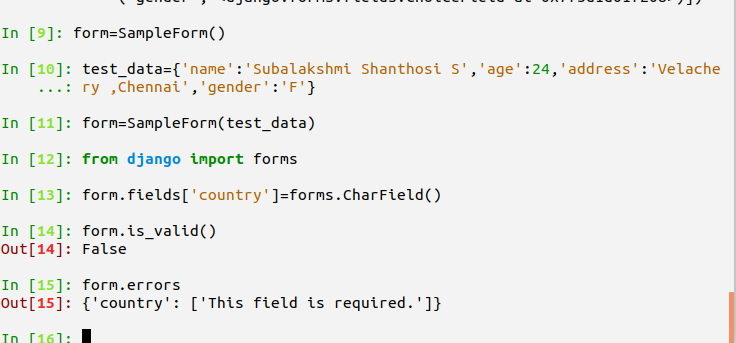
\includegraphics[scale=0.55]{project/includingFieldsForm.png}
\newpage
\subsection{Running Migration}

Migrations are Django's way of propagating changes you make to your models (adding a field, deleting a model,
etc.) into your database schema. They're designed to be mostly automatic, but you'll need to know when to make
migrations, when to run them, and the common problems you might run into.\\

There are several commands which you will use to interact with migrations and Django's handling of database schema:
\begin{enumerate}
	\item \textbf{migrate}, which is responsible for applying and unapplying migrations.
	\item \textbf{makemigrations}, which is responsible for creating new migrations based on the changes you have made to your models.
	\item \textbf{sqlmigrate}, which displays the SQL statements for a migration.
	\item \textbf{showmigrations}, which lists a project's migrations and their status.
\end{enumerate}
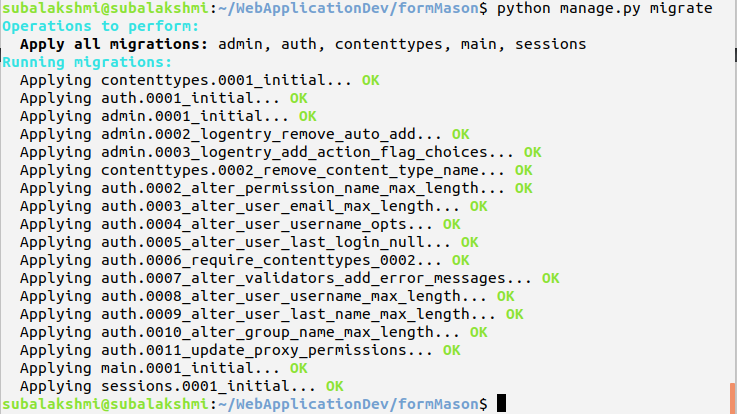
\includegraphics[scale=0.55]{project/migrationRunning.png}\\

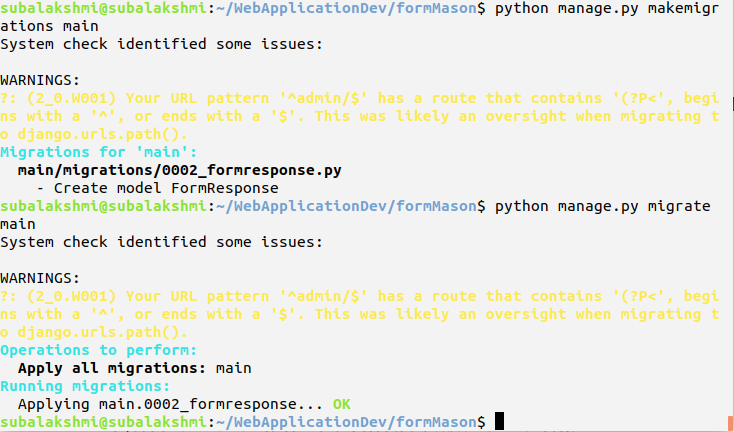
\includegraphics[scale=0.55]{project/savingRespMigration.png}
\subsection{Using created Model}
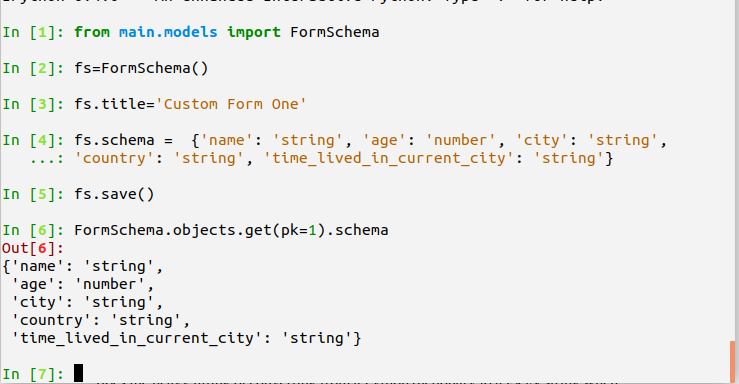
\includegraphics[scale=0.45]{project/formSchemaDefn.png}

\chapter{Forms in Django}
\section{Introduction}
\paragraph{} Django provides a rich framework to facilitate the creation of forms and the manipulation of form data.
\begin{itemize}
	\item \textbf{The basics:} 
	\begin{itemize}
		\item Overview 
		\item Form API 
		\item Built-in fields 
		\item Built-in widgets
	\end{itemize}
   \item \textbf{Advanced:}
   \begin{itemize}
   	\item Forms for models 
   	\item Integrating media  
   	\item Formsets 
   	\item Customizing validation
   \end{itemize}
\end{itemize}
\subsection{Django's role in forms}
Django handles three distinct parts of the work involved in forms:\\
\begin{itemize}
	\item Preparing and Restructuring data to make it ready for rendering.
	\item Creating HTML forms for the data.
	\item Receiving and Processing submitted forms and data from the client.
\end{itemize}
\subsection{Forms in Django}
\subsubsection{ The Django \textbf{Form} class:}
Django Model describes the logical \textbf{structure} of an object, it's \textbf{behavior}, and the way its parts are represented to us, a Form class describes a form and determines how it works and appears.\\

In a similar way that a model class's fields map to database fields, a form class's fields map to HTML form <input> elements. (A \textbf{ModelForm} maps a model class's fields to HTML form <input> elements via a Form; this is what the Django admin is based upon.)\\

A form's fields are themselves classes; they manage form data and perform validation when a form is submitted. A DateField and a FileField handle very different kinds of data and have to do different things with it.\\

A form field is represented to a user in the browser as an HTML "\textbf{widget}" - a piece of user interface machinery. Each field type has an appropriate default Widget class, but these can be overridden as required.

\subsubsection{Instantiating, processing, and rendering forms}
While \textbf{rendering} a form:
\begin{itemize}
	\item Get hold of it in the view (fetch it from the database, for example).
	\item Pass it to the template context.
	\item Expand it to HTML markup using template variables.	
\end{itemize}
When we \textbf{instantiate} a form, we can opt to leave it empty or pre-populate it, for example with:
\begin{itemize}
	\item Data from a saved model instance (as in the case of admin forms for editing).
	\item Data that we have collated from other sources.
	\item Data received from a previous HTML form submission.	
\end{itemize}
\newpage
\section{Form Field Types}
\paragraph{}Each model field has a corresponding default form field. For example, a CharField on a model is represented as a CharField on a form. A model ManyToManyField is represented as a MultipleChoiceField.

\begin{table}[]
	\begin{tabular}{|l|l|ll}
		\cline{1-2}
		\textbf{Model Field} & \textbf{Form Field}       &  &  \\ \cline{1-2}
		AutoField            & Not represented in form   &  &  \\ \cline{1-2}
		BigAutoField         & Not represented in form   &  &  \\ \cline{1-2}
		BigIntegerField      & IntegerField              &  &  \\ \cline{1-2}
		BinaryField          & CharField - True or false &  &  \\ \cline{1-2}
		BooleanField         & BooleanField              &  &  \\ \cline{1-2}
		CharField            & CharField                 &  &  \\ \cline{1-2}
		DateField            & DateField                 &  &  \\ \cline{1-2}
		ForeignKey           & ModelChoiceField          &  &  \\ \cline{1-2}
		ManyToManyField      & ModelMultipleChoiceField  &  &  \\ \cline{1-2}
		TextField            & CharField                 &  &  \\ \cline{1-2}
	\end{tabular}
\caption{Conversion of Model to Form Fields }
\label{tab:my-table}
\end{table}
\subsection{Accessing the fields from the form}
Using command \textbf{Form.fields}
\begin{lstlisting}[language=python,numbers=none]
>>> f.as_table().split('\n')[0]
'<tr><th>Name:</th><td><input name="name" type="text" value="instance" required></td></tr>'
>>> f.fields['name'].label = "Username"
>>> f.as_table().split('\n')[0]
'<tr><th>Username:</th><td><input name="name" type="text" value="instance" required></td></tr>
\end{lstlisting}

\subsection{Outputting forms as HTML}
The second task of a Form object is to render itself as HTML. To do so, simply print it:
\begin{itemize}
	\item \textbf{Form.as\_p()}:\\
	as\_p() renders the form as a series of \textbf{<p>} tags, with each <p> containing one field.
	\item \textbf{Form.as\_ul()}: Similarly,Render with series of \textbf{<ul>} tags.
	\item \textbf{Form.as\_table()}:Renders as HTML table.
\end{itemize}
\newpage
\section{Forms in FormMason}
Form with inplace vaildation based on the field type and additional parameters such as max-length,min-length,required etc. specified on Form Fieldtype constructor.\\
\begin{lstlisting}[language=python,numbers=none]
# Form class which inherits django forms. Consists of four fields Name,Age,Address and Gender
from django import forms
class SampleForm(forms.Form):
	name = forms.CharField()
	age = forms.IntegerField()
	address = forms.CharField(required=False)
	gender = forms.ChoiceField(choices=(('M', 'Male'),('F','Female')))
\end{lstlisting}
\subsubsection{Use of Ordered Dict Type in Django}
Unlike the traditional Dictonary - the fields of Form are of type Ordered Dictionary.\\
This is to \textbf{preserve} the order of insertion of field while writing forms.py.

\subsection{Customised Form}
New Dynamic Form(NewDynamicFormForm class) with the following fields as class members:
\begin{enumerate}
\item \textbf{form\_pk} : CharField - required : False, HiddenInput.
\item \textbf{title} : CharField - required : True, Normal Input.
\item \textbf{schema} : CharField - required : True, Normal Input.
\item Method \textbf{clean\_schema} : To trying loading json schema and returning schema.
\end{enumerate}
\newpage
\begin{lstlisting}[language=python,numbers=none]
 import json
 from django import forms
 from django.db.models.functions import Lower,Upper
 
 # Form fields - JSON data and title.
 class NewDynamicFormForm(forms.Form):
 	form_pk=forms.CharField(widget=forms.HiddenInput(),required=False)
 	title = forms.CharField()
 	schema = forms.CharField(widget=forms.Textarea()) 
 # Method to load the JSON schema
 def clean_schema(self):
 	schema = self.cleaned_data["schema"]
 	schema = json.loads(schema)
 	return schema
\end{lstlisting}
$\bullet${Alteration in views and template}
\begin{lstlisting}[language=python,numbers=none]
#Create Edit Form View to load data from JSON into created model
class CreateEditFormView(FormView):
	form_class = NewDynamicFormForm
	template_name = "create_edit_form.html"
	def get_initial(self):
		if "form_pk" in self.kwargs:
			form = FormSchema.objects.get(pk=self.kwargs["form_pk"])
			initial = {
				"form_pk": form.pk,
				"title": form.title,
				"schema": json.dumps(form.schema)
			}
		else:
			initial = {}  # Ensure backward compactibility of old form layout
	return initial
# Get context data - Form context
def get_context_data(self, **kwargs):
	ctx = super(CreateEditFormView, self).get_context_data(**kwargs)
	if "form_pk" in self.kwargs:
		ctx["form_pk"] = self.kwargs["form_pk"]
	return ctx
# Save old or new form fields.
def form_valid(self, form):
	cleaned_data = form.cleaned_data
	if cleaned_data.get("form_pk"):
		old_form = FormSchema.objects.get(pk=cleaned_data["form_pk"])
		old_form.title = cleaned_data["title"]
		old_form.schema = cleaned_data["schema"]
		old_form.save()
	else:
		new_form = FormSchema(title=cleaned_data["title"],schema=cleaned_data["schema"])
		new_form.save()
		return HttpResponseRedirect(reverse("home"))
\end{lstlisting}
\begin{lstlisting}[language=html,numbers=none]
<!-- Changes to include link for edit form -- >
<! -- create_edit_form.html-->


<h1>Create/Edit Form</h1>

<li>
<form action="" method="post">

</li>

<li>
<form action="" method="post">

</li>
{{ form.as_p }}
<li>
<input type="submit" value="Create Form" />
</li>
</form>

\end{lstlisting}
\chapter{Implementation}
\paragraph{}WRITE HERE, PARAGRAPH 1.
\paragraph{}WRITE HERE, PARAGRAPH 2.

\begin{figure}[H]
  \centering
    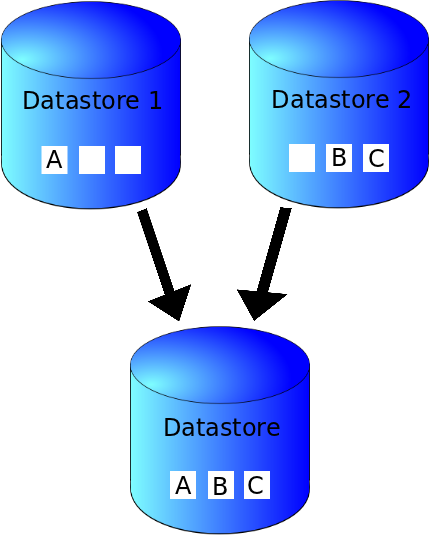
\includegraphics[scale=0.5]{project/images/data-sync}
  \caption{\textbf{IMAGE CAPTION}}
\end{figure}

\begin{lstlisting}
  PASTE YOUR CODE HERE
\end{lstlisting}
\newpage


\chapter{Screenshots of Project}
\section{SECTION NAME}
\vspace{2cm}
\begin{figure}[H]
  \centering
    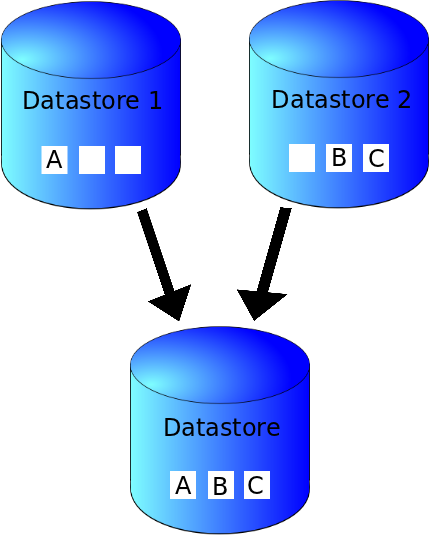
\includegraphics[height= 11cm, width=17cm]{project/images/data-sync}
\end{figure}
\newpage
\begin{figure}[H]
  \centering
    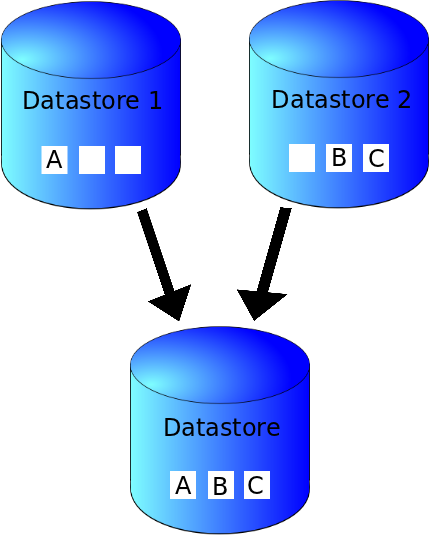
\includegraphics[height= 11cm, width=17cm]{project/images/data-sync}
\end{figure}
\vspace{1cm}
\begin{figure}[H]
  \centering
    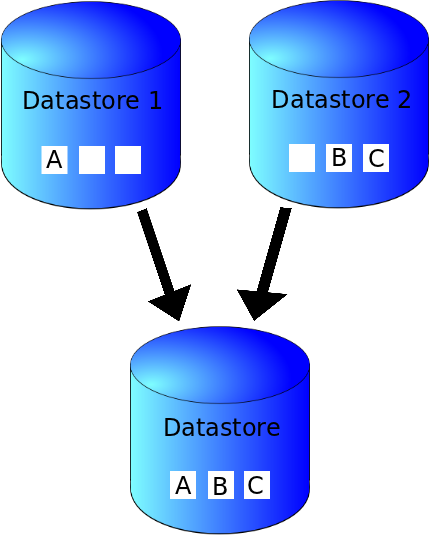
\includegraphics[height= 11cm, width=17cm]{project/images/data-sync}
\end{figure}
\chapter{Conclusion and Future Scope}
\section{Conclusion}
\paragraph{}WRITE HERE.
\section{Future Scope}
\paragraph{}WRITE HERE.
\begin{itemize}
 \item ITEM 1
 \item ITEM 2
 \item ITEM 3
\end{itemize} % adds the Scheduling and Planning page
\addcontentsline{toc}{chapter}{References}
\begin{thebibliography}{99}
\bibitem{WRITE A SHORT-NAME WITHOUT SPACE} \emph{NAME OF IEEE PAPER}; NAME OF AUTHORS
\bibitem{ChapterFour:Introduction to Django Models} \href{https://buildmedia.readthedocs.org/media/pdf/django/latest/django.pdf}{Django documentation}
\end{thebibliography} % adds the References page

\end{document}